
\de{ĐỀ THI HỌC KỲ I NĂM HỌC 2022-2023}{Trường THPT Yên Mô B - Quảng Bình}
\begin{center}
	\textbf{PHẦN 1 - TRẮC NGHIỆM}
\end{center}
\Opensolutionfile{ans}[ans/ans]
\begin{ex}%[0D1Y1-3]%[Dự án đề kiểm tra HKI NH22-23-VU Ngoc Hao]%[ĐỀ KIỂM TRA CUỐI HỌC KỲ I TRƯỜNG THPT YÊN MÔ B-NINH BÌNH]
Mệnh đề phủ định của mệnh đề $P\colon$\lq\lq$\exists x\in\mathbb{R},\,x^2-10=0$\rq\rq là
		\choice
	{$\overline{P}\colon$\lq\lq$\forall x \in\mathbb{R},\,x^2-10 \leq 0$\rq\rq}
	{$\overline{P}\colon$\lq\lq$\exists x \in\mathbb{R},\,x^2-10 \neq 0$\rq\rq}
	{$\overline{P}\colon$\lq\lq$\forall x \in\mathbb{R},\,x^2-10=0$\rq\rq}
	{\True $\overline{P}\colon$\lq\lq$\forall x\in \mathbb{R},\, x^2-10\neq 0$\rq\rq}
		\loigiai{
Phủ định của mệnh đề $P$ là $\overline{P}\colon$\lq\lq$\forall x\in\mathbb{R},\,x^2-10\neq 0$\rq\rq.
}
\end{ex}

\begin{ex}%[0D1B3-1]%[Dự án đề kiểm tra HKI NH22-23-VU Ngoc Hao]%[ĐỀ KIỂM TRA CUỐI HỌC KỲ I TRƯỜNG THPT YÊN MÔ B-NINH BÌNH]
Cho hai tập hợp $A=[-4;4]$, $B=(0;6)$. Tìm $A\cap B$.
		\choice
	{\True $A\cap B=(0;4]$}
	{$A\cap B=(0;4)$}
	{$A\cap B=[0;4]$}
	{$A\cap B=[-4;6)$}
		\loigiai{
Ta thấy $A\cap B=(0;4]$.
}
\end{ex}

\begin{ex}%[0D1B3-1]%[Dự án đề kiểm tra HKI NH22-23-VU Ngoc Hao]%[ĐỀ KIỂM TRA CUỐI HỌC KỲ I TRƯỜNG THPT YÊN MÔ B-NINH BÌNH]
Cho hai tập hợp $A=\left\{x\in\mathbb{R}\mid x^2-3x+2=0\right\}$, $B=\{1;3;5;7;9\}$. Tìm $A\cup B$.
		\choice
	{\True $A\cup B=\{1;2;3;5;7;9\}$}
	{$A\cup B=\{1;3;5;7;9\}$}
	{$A\cup B=\{3;5;7;9\}$}
	{$A\cup B=\{1\}$}
		\loigiai{
Ta có $x^2-3x+2=0\Leftrightarrow\hoac{&x=1\\&x=2.}$\\
Suy ra $A=\left\{1;2\right\}$.\\
Khi đó $A\cup B=\{1;2;3;5;7;9\}$.
}
\end{ex}

\begin{ex}%[0D2Y1-3]%[Dự án đề kiểm tra HKI NH22-23-VU Ngoc Hao]%[ĐỀ KIỂM TRA CUỐI HỌC KỲ I TRƯỜNG THPT YÊN MÔ B-NINH BÌNH]
Tìm tất cả các giá trị của tham số $m$ để hàm số $y=(m-1)x+m$ đồng biến trên $\mathbb{R}$.
		\choice
	{$m<1$}
	{\True $m>1$}
	{$m>0$}
	{$m\geq 1$}
		\loigiai{
Hàm số đã cho có dạng $y=ax+b$ đồng biến khi $a>0$ nên ta có $m-1>0\Leftrightarrow m>1$.
}
\end{ex}

\begin{ex}%[0D2Y1-2]%[Dự án đề kiểm tra HKI NH22-23-VU Ngoc Hao]%[ĐỀ KIỂM TRA CUỐI HỌC KỲ I TRƯỜNG THPT YÊN MÔ B-NINH BÌNH]
Tìm tập xác định của hàm số $y=\dfrac{2x-3}{x+1}$.
		\choice
	{$\mathscr D=\mathbb{R}\setminus\{1\}$}
	{\True $\mathscr D=\mathbb{R}\setminus\{-1\}$}
	{$\mathscr D=\mathbb{R}$}
	{$\mathscr D=\mathbb{R}\setminus\{0\}$}
		\loigiai{
Điều kiện xác định $x+1\neq0\Leftrightarrow x\neq-1$.\\
Tập xác định $\mathscr D=\mathbb{R}\setminus\{-1\}$.
}
\end{ex}

\begin{ex}%[0D4Y2-3]%[Dự án đề kiểm tra HKI NH22-23-VU Ngoc Hao]%[ĐỀ KIỂM TRA CUỐI HỌC KỲ I TRƯỜNG THPT YÊN MÔ B-NINH BÌNH]%Câu 6
Điểm nào sau đây thuộc miền nghiệm của bất phương trình $3x-y\geq 2$?
		\choice
	{$A(1;3)$}
	{$B(2;5)$}
	{\True $C(3;4)$}
	{$D(0;1)$}
		\loigiai{
Ta thấy điểm $C(3;4)$ thuộc miền nghiệm của bất phương trình vì $3\cdot4-4\geq2$ thỏa mãn.
}
\end{ex}

\begin{ex}%[0D4Y2-3]%[Dự án đề kiểm tra HKI NH22-23-VU Ngoc Hao]%[ĐỀ KIỂM TRA CUỐI HỌC KỲ I TRƯỜNG THPT YÊN MÔ B-NINH BÌNH]%Câu 7
\immini{Nửa mặt phẳng không bị gạch hình bên (tính cả bờ) biểu diễn miền nghiệm của bất phương trình nào sau đây?
		\choice
	{$x+y\geq 2$}
	{$x+y\leq 2$}
	{$x-y\leq 2$}
	{\True $x-y\geq 2$}
}{		
\begin{tikzpicture}[scale=0.8, line join=round, font=\footnotesize, line cap=round,>=stealth]
\fill[pattern=north east lines](-1,-3)--(4,2)--(-1,2)--cycle;
\draw[-stealth](-1,0)--(4,0) node[above]{$x$}; 
\draw[-stealth](0,-3)--(0,2) node[below right]{$y$};		
\draw[fill=black](0,0)circle (1pt)node[below left]{$O$};
\foreach \x/\g in {2/-60}\fill[black] (\x,0) circle (1pt)+(\g:.4)node{$\x$};
\foreach \x/\g in {-2/-20}\fill[black] (0,\x) circle (1pt)+(\g:.4)node{$\x$};		
\draw[smooth,domain=-1:4] plot (\x,{\x-2})node[right]{$d$};
\end{tikzpicture}
}
\loigiai{
Ta thấy bờ là đường thẳng đi qua các điểm $(2;0)$, $(0;-2)$ và miền nghiệm không chứa gốc tọa độ nên bất phương trình đó là $x-y\geq 2$.
}
\end{ex}

\begin{ex}%[0D4B2-4]%[Dự án đề kiểm tra HKI NH22-23-VU Ngoc Hao]%[ĐỀ KIỂM TRA CUỐI HỌC KỲ I TRƯỜNG THPT YÊN MÔ B-NINH BÌNH]%Câu 8
Miền nghiệm của hệ bất phương trình $\heva{&x\geq 1\\&y\geq 0\\&x+y\leq 4\\&x-y\leq1}$ là
		\choice
	{một nửa mặt phẳng}
	{\True miền tam giác}
	{miền tứ giác}
	{miền ngũ giác}
		\loigiai{
\immini{
$\heva{&x\geq 1&(1)\\&y\geq 0&(2)\\&x+y\leq 4&(3)\\&x-y\leq1&(4)}$\\
Ta vẽ các bờ\\
$\heva{&x=1&(d_1)\\&y=0&(d_2)\\&x+y=4&(d_3)\\&x-y=1&(d_4).}$\\
Gọi $A=d_1\cap d_3$, $B=d_1\cap d_4$, $A=d_3\cap d_4$.
}{
\begin{tikzpicture}[scale=1, line join=round, font=\footnotesize, line cap=round,>=stealth]
\fill[pattern=north east lines,opacity=0.5](-1,-1)--(1,-1)--(1,4.5)--(-1,4.5)--cycle;
\fill[pattern=north east lines,opacity=0.5](-1,0)--(4.4,0)--(4.5,-1)--(-1,-1)--cycle;
\fill[pattern=north east lines,opacity=0.5](-1,0)--(4.5,0)--(4.5,-1)--(-1,-1)--cycle;
\fill[pattern=north east lines,opacity=0.5](0,-1)--(4.5,-1)--(4.5,3.5)--cycle;
\fill[pattern=north east lines,opacity=0.5](0,4)--(4,0)--(4.5,0)--(4.5,4.5)--(0,4.5)--cycle;
\draw[-stealth](-1,0)--(4.5,0) node[above]{$x$}; 
\draw[-stealth](0,-1)--(0,4.5) node[below right]{$y$};		
\draw[fill=black](0,0)circle (1pt)node[below left]{$O$};
\foreach \x/\g in {1/-30,4/-90}\fill[black] (\x,0) circle (1pt)+(\g:.4)node{$\x$};
\foreach \x/\g in {-1/150,4/180}\fill[black] (0,\x) circle (1pt)+(\g:.4)node{$\x$};
\path
(1,0) coordinate (A)
(1,3) coordinate (B)
(2.5,1.5) coordinate (C)
;
\foreach \x/\g in {A/150,B/180,C/0}\fill[black] (\x) circle(1pt)+(\g:0.3)node{$\x$};			
\draw[smooth,domain=-0.5:4.5] plot (\x,{-\x+4});
\draw[smooth,domain=0:4.5] plot (\x,{\x-1});
\draw (1,-1)--(1,4.5);
\end{tikzpicture}
}
\noindent Ta thấy $M(0;1)\notin (1)$, $M(0;1)\in (2)$, $M(0;1)\in (3)$, $M(0;1)\in (4)$.\\
Dựa vào điểm $M$ trên ta có miền nghiệm của hệ bất phương trình là miền trong của tam giác $ABC$ và các cạnh của tam giác $ABC$.
}
\end{ex}

\begin{ex}%[0D5B3-1]%[Dự án đề kiểm tra HKI NH22-23-VU Ngoc Hao]%[ĐỀ KIỂM TRA CUỐI HỌC KỲ I TRƯỜNG THPT YÊN MÔ B-NINH BÌNH]%Câu 9
Điểm thi cuối Học kì I của bạn An được thống kê như sau
\begin{center}
\begin{tabular}{|c|c|c|c|c|c|c|c|c|}
\hline Môn & Toán & Lý & Hóa & Sinh & Văn & Anh & Sử & Tin \\
\hline Điểm & $9{,}0$ & $8{,}5$ & $9{,}0$ & $7{,}5$ & $8{,}0$ & $7{,}5$ & $7{,}0$ & $8{,}5$ \\
\hline
\end{tabular}
\end{center}
Trung vị của mẫu số liệu trên là
		\choice
	{$7{,}75$}
	{$8{,}0$}
	{\True $8{,}25$}
	{$8{,}5$}
		\loigiai{
Mẫu số liệu được sắp xếp lại theo điểm từ bé đến lớn là
\begin{center}
\begin{tabular}{|c|c|c|c|c|c|c|c|c|}
\hline Môn & Sử & Sinh & Anh & Văn & Lý & Tin & Toán & Hóa\\
\hline Điểm & $7{,}0$ & $7{,}5$ & $7{,}5$ & $8{,}0$ & $8{,}5$ & $8{,}5$ & $9{,}0$ & $9{,}0$\\
\hline
\end{tabular}
\end{center}
$\mathrm M_e=\dfrac{1}{2}\left(8{,}0+8{,}5\right)=8{,}25$.
}
\end{ex}

\begin{ex}%[0D5B4-1]%[Dự án đề kiểm tra HKI NH22-23-VU Ngoc Hao]%[ĐỀ KIỂM TRA CUỐI HỌC KỲ I TRƯỜNG THPT YÊN MÔ B-NINH BÌNH]%Câu 10
Điểm thi cuối Học kì I của bạn An được thống kê như sau
\begin{center}
\begin{tabular}{|c|c|c|c|c|c|c|c|c|}
\hline Môn & Toán & Lý & Hóa & Sinh & Văn & Anh & Sử & Tin \\
\hline Điểm & $9{,}0$ & $8{,}5$ & $9{,}0$ & $7{,}5$ & $8{,}0$ & $7{,}5$ & $7{,}0$ & $8{,}5$\\
\hline
\end{tabular}
\end{center}
Độ lệch chuẩn của mẫu số liệu trên gần nhất với số nào dưới đây?
		\choice
	{$0{,}6$}
	{\True $0{,}7$}
	{$0{,}8$}
	{$0{,}9$}
		\loigiai{
Điểm trung bình $\overline{x}=\dfrac{9{,}0+8{,}5+9{,}0+7{,}5+8{,}0+7{,}5+7{,}0+8{,}5}{8}=8{,}125$.\\
$s^2=\dfrac{1}{8}\left(9{,}0^2+8{,}5^2+9{,}0^2+7{,}5^2+8{,}0^2+7{,}5^2+7{,}0^2+8{,}5^2\right)-8{,}125^2\approx0{,}48$.\\
Độ lệch chuẩn $s=\sqrt{0{,}48}\approx0{,}7$.
}
\end{ex}

\begin{ex}%[0H2B1-2]%[Dự án đề kiểm tra HKI NH22-23-VU Ngoc Hao]%[ĐỀ KIỂM TRA CUỐI HỌC KỲ I TRƯỜNG THPT YÊN MÔ B-NINH BÌNH]%Câu 11
Cho góc $\alpha$ biết $\sin\alpha=\dfrac{3}{5}$, $0^{\circ}<\alpha<90^{\circ}$. Tính $\cos\alpha$.
		\choice
	{$\cos\alpha=\dfrac{16}{25}$}
	{\True $\cos\alpha=\dfrac{4}{5}$}
	{$\cos\alpha=-\dfrac{4}{5}$}
	{$\cos\alpha=\dfrac{2}{5}$}
		\loigiai{
Ta có $\cos^2\alpha=1-\sin^2\alpha=1-\left(\dfrac{3}{5}\right)^2=\dfrac{16}{25}\Rightarrow\cos\alpha=\dfrac{4}{5}$ (vì $0^{\circ}<\alpha<90^{\circ}$).
}
\end{ex}

\begin{ex}%[0H2B3-4]%[Dự án đề kiểm tra HKI NH22-23-VU Ngoc Hao]%[ĐỀ KIỂM TRA CUỐI HỌC KỲ I TRƯỜNG THPT YÊN MÔ B-NINH BÌNH]%Câu 12
Cho tam giác $ABC$ biết $BC=6$; $A=120^{\circ}$. Tính bán kính $R$ của đường tròn ngoại tiếp tam giác $ABC$.
		\choice
	{\True $R=2\sqrt{3}$}
	{$R=6$}
	{$R=12$}
	{$R=4\sqrt{3}$}
		\loigiai{
Áp dụng định lý sin ta có $R=\dfrac{BC}{2\sin A}=\dfrac{6}{2\cdot\frac{\sqrt{3}}{2}}=2\sqrt{3}$.
}
\end{ex}

\begin{ex}%[0H2B3-4]%[Dự án đề kiểm tra HKI NH22-23-VU Ngoc Hao]%[ĐỀ KIỂM TRA CUỐI HỌC KỲ I TRƯỜNG THPT YÊN MÔ B-NINH BÌNH]%Câu 13
Cho tam giác $ABC$, biết $a=4$; $c=5$; $\widehat{B}=60^{\circ}$. Tính cạnh $b$.
		\choice
	{$b=21$}
	{\True $b=\sqrt{21}$}
	{$b=31$}
	{$b=\sqrt{31}$}
		\loigiai{
Áp dụng định lý cosin ta có $b^2=a^2+c^2-2ac\cdot\cos B=16+25-2\cdot4\cdot5\cdot\dfrac{1}{2}=21$.\\
Suy ra $b=\sqrt{21}$.
}
\end{ex}

\begin{ex}%[0H2B3-4]%[Dự án đề kiểm tra HKI NH22-23-VU Ngoc Hao]%[ĐỀ KIỂM TRA CUỐI HỌC KỲ I TRƯỜNG THPT YÊN MÔ B-NINH BÌNH]%Câu 14
Tính diện tích $S$ của tam giác $ABC$, biết $a=4$; $b=3$; $\widehat{C}=30^{\circ}$ .
		\choice
	{$S=6\sqrt{3}$}
	{$S=6$}
	{$S=3\sqrt{3}$}
	{\True $S=3$}
		\loigiai{
Ta có $S=\dfrac{1}{2}ab\cdot\sin C=\dfrac{1}{2}\cdot4\cdot3\cdot\dfrac{1}{2}=3$.
}
\end{ex}

\begin{ex}%[0H2B3-4]%[Dự án đề kiểm tra HKI NH22-23-VU Ngoc Hao]%[ĐỀ KIỂM TRA CUỐI HỌC KỲ I TRƯỜNG THPT YÊN MÔ B-NINH BÌNH]%Câu 15
Cho tam giác $ABC$ có trọng tâm $G$. Gọi $I$ là trung điểm của đoạn $AB$, điểm $M$ bất kỳ. Khẳng định nào sau đây \textbf{sai}?
		\choice
	{$\overrightarrow{IA}+\overrightarrow{IB}=\overrightarrow{0}$}
	{$\overrightarrow{MA}+\overrightarrow{MB}=2\overrightarrow{MI}$}
	{\True $\overrightarrow{IA}=\overrightarrow{IB}$}
	{$\overrightarrow{GA}+\overrightarrow{GB}+\overrightarrow{GC}=\overrightarrow{0}$}
		\loigiai{
Ta có $\overrightarrow{IA}+\overrightarrow{IB}=\overrightarrow{0}\Leftrightarrow\overrightarrow{IA}=-\overrightarrow{IB}$. Do đó, $\overrightarrow{IA}=\overrightarrow{IB}$ là mệnh đề sai. 
}
\end{ex}

\begin{ex}%[0H1B3-2]%[Dự án đề kiểm tra HKI NH22-23-VU Ngoc Hao]%[ĐỀ KIỂM TRA CUỐI HỌC KỲ I TRƯỜNG THPT YÊN MÔ B-NINH BÌNH]%Câu 16
Cho tam giác $ABC$ đều, có cạnh bằng $4$. Véc-tơ $\overrightarrow{u}=\overrightarrow{AB}-\overrightarrow{AC}$ có độ dài là
		\choice
	{$2$}
	{\True $4$}
	{$0$}
	{$2\sqrt{3}$}
		\loigiai{
Ta có $\overrightarrow{u}=\overrightarrow{AB}-\overrightarrow{AC}=\overrightarrow{CB}\Rightarrow \left|\overrightarrow{u}\right|=\left|\overrightarrow{CB}\right|=4$.
}
\end{ex}

\begin{ex}%[0H1Y4-3]%[Dự án đề kiểm tra HKI NH22-23-VU Ngoc Hao]%[ĐỀ KIỂM TRA CUỐI HỌC KỲ I TRƯỜNG THPT YÊN MÔ B-NINH BÌNH]%Câu 17
Trong mặt phẳng tọa độ $Oxy$, cho $\overrightarrow{a}=(1;2)$, $\overrightarrow{b}=(3;-4)$. Tìm tọa độ của $\overrightarrow{u}=\overrightarrow{a}+\overrightarrow{b}$.
		\choice
	{$\overrightarrow{u}=(2;-6)$}
	{$\overrightarrow{u}=(-2;6)$}
	{$\overrightarrow{u}=(3;-8)$}
	{\True $\overrightarrow{u}=(4;-2)$}
		\loigiai{
Ta có $\overrightarrow{u}=\overrightarrow{a}+\overrightarrow{b}=(1+3;3-4)=(4;-2)$.
}
\end{ex}

\begin{ex}%[0H1B4-3]%[Dự án đề kiểm tra HKI NH22-23-VU Ngoc Hao]%[ĐỀ KIỂM TRA CUỐI HỌC KỲ I TRƯỜNG THPT YÊN MÔ B-NINH BÌNH]%Câu 18
Trong mặt phẳng tọa độ $Oxy$, cho $A(1;2)$, $B(3;1)$. Tính độ dài đoạn thẳng $AB$.
		\choice
	{$AB=3$}
	{$AB=\sqrt{3}$}
	{$AB=5$}
	{\True $AB=\sqrt{5}$}
		\loigiai{
Ta có $\overrightarrow{AB}=(2;-1)\Rightarrow AB=\sqrt{2^2+(-1)^2}=\sqrt{5}$.
}
\end{ex}

\begin{ex}%[0H1Y4-3]%[Dự án đề kiểm tra HKI NH22-23-VU Ngoc Hao]%[ĐỀ KIỂM TRA CUỐI HỌC KỲ I TRƯỜNG THPT YÊN MÔ B-NINH BÌNH]%Câu 19
Trong mặt phẳng tọa độ $Oxy$, cho biết $A(1;2)$, $B(3;-4)$. Tìm tọa độ trung điểm $I$ của đoạn $AB$.
		\choice
	{$I(4;-2)$}
	{\True $I(2;-1)$}
	{$I(1;-3)$}
	{$I(2;-6)$}
		\loigiai{
Tọa độ trung điểm của $AB$ là $\heva{&x_I=\dfrac{x_A+x_B}{2}=\dfrac{1+3}{2}=2\\&y_I=\dfrac{y_A+y_B}{2}=\dfrac{2-4}{2}=-1.}$\\
Vậy $I(2;-1)$.
}
\end{ex}

\begin{ex}%[0D2Y3-4]%[Dự án đề kiểm tra HKI NH22-23-VU Ngoc Hao]%[ĐỀ KIỂM TRA CUỐI HỌC KỲ I TRƯỜNG THPT YÊN MÔ B-NINH BÌNH]%Câu 20
\immini{Cho hàm số $y=f(x)$ có đồ thị như hình bên. Số nghiệm của phương trình $f(x)-1=0$ là
		\choice
	{$0$}
	{$1$}
	{\True $2$}
	{$3$}
}{
\begin{tikzpicture}[scale=0.75, line join=round, font=\footnotesize, line cap=round,>=stealth]
\draw[-stealth](-1,0)--(4,0) node[above]{$x$}; 
\draw[-stealth](0,-1.5)--(0,4) node[below right]{$y$};		
\draw[fill=black](0,0)circle (1pt)node[below left]{$O$};
\draw[dashed](0,-1)-|(2,0);
\foreach \x/\g in {-1/180}\fill[black] (0,\x) circle (1pt)+(\g:.4)node{$\x$};		
\draw[smooth,domain=-0.2:4.2] plot (\x,{(\x)^2-4*\x+3});
\end{tikzpicture}
}
		\loigiai{
\immini{
$f(x)-1=0\Leftrightarrow f(x)=1$.\\
Dựa vào đồ thị ta thấy đường thẳng $f(x)=1$ cắt đồ thị tại hai điểm phân biệt. Nên phương trình có hai nghiệm phân biệt.
}{
\begin{tikzpicture}[scale=0.75, line join=round, font=\footnotesize, line cap=round,>=stealth]
\draw[-stealth](-1,0)--(4,0) node[above]{$x$}; 
\draw[-stealth](0,-1.5)--(0,4) node[below right]{$y$};		
\draw[fill=black](0,0)circle (1pt)node[below left]{$O$};
\draw[dashed](0,-1)-|(2,0);
\foreach \x/\g in {-1/180,1/150}\fill[black] (0,\x) circle (1pt)+(\g:.4)node{$\x$};		
\draw[smooth,domain=-0.2:4.2] plot (\x,{(\x)^2-4*\x+3});
\draw[smooth,domain=-0.8:4] plot (\x,{1})node[above right]{$f(x)=1$};
\end{tikzpicture}
}
}
\end{ex}

\begin{ex}%[0D2Y3-1]%[Dự án đề kiểm tra HKI NH22-23-VU Ngoc Hao]%[ĐỀ KIỂM TRA CUỐI HỌC KỲ I TRƯỜNG THPT YÊN MÔ B-NINH BÌNH]%Câu 21
Cho hàm số $y=x^2-6x+10$. Khẳng định nào sau đây đúng?
		\choice
	{Hàm số đồng biến trên khoảng $(-\infty;3)$, nghịch biến trên khoảng $(3;+\infty)$}
	{Hàm số đồng biến trên khoảng $(-\infty;-3)$, nghịch biến trên khoảng $(-3;+\infty)$}
	{\True Hàm số nghịch biến trên khoảng $(-\infty;3)$, đồng biến trên khoảng $(3;+\infty)$}
	{Hàm số nghịch biến trên khoảng $(-\infty;-3)$, đồng biến trên khoảng $(-3;+\infty)$}
		\loigiai{
Hàm số có $a=1>0$ nên nghịch biến trên khoảng $\left(-\infty;\dfrac{-b}{2a}\right)=(-\infty;3)$, đồng biến trên khoảng $\left(\dfrac{-b}{2a};+\infty\right)=(3;+\infty)$.
}
\end{ex}

\begin{ex}%[0D2B3-4]%[Dự án đề kiểm tra HKI NH22-23-VU Ngoc Hao]%[ĐỀ KIỂM TRA CUỐI HỌC KỲ I TRƯỜNG THPT YÊN MÔ B-NINH BÌNH]%Câu 22
Biết Parabol $(P)\colon y=x^2-2x-3$ cắt đường thẳng $d\colon y=5x-1$ tại hai điểm phân biệt có hoành độ $x_1$, $x_2$. Tính giá trị của biểu thức $Q=x_1^2+x_2^2+10\left(x_1+x_2\right)$.
		\choice
	{\True $Q=123$}
	{$Q=105$}
	{$Q=-17$}
	{$Q=-30$}
		\loigiai{
Phương trình hoành độ giao điểm của $(P)$ và $(d)$\\
$x^2-2x-3=5x-1\Leftrightarrow x^2-7x-2=0$ có hai nghiệm phân biệt vì $a$, $c$ trái dấu.\\
Khi đó $S=x_1+x_2=-\dfrac{b}{a}=7$, $P=x_1x_2=\dfrac{c}{a}=-2$.\\
$Q=x_1^2+x_2^2+10\left(x_1+x_2\right)=S^2-2P+10S=49+4+70=123$.
}
\end{ex}

\begin{ex}%[0D3B2-4]%[Dự án đề kiểm tra HKI NH22-23-VU Ngoc Hao]%[ĐỀ KIỂM TRA CUỐI HỌC KỲ I TRƯỜNG THPT YÊN MÔ B-NINH BÌNH]%Câu 23
Tập nghiệm của phương trình $\sqrt{2x^2-6x-8}=\sqrt{x^2-5x-2}$ là
		\choice
	{\True $\{-2\}$}
	{$\{3\}$}
	{$\{-2;3\}$}
	{$\varnothing$}
		\loigiai{
\begin{eqnarray*}
&&\sqrt{2x^2-6x-8}=\sqrt{x^2-5x-2}\\
&\Leftrightarrow&\heva{&2x^2-6x-8\geq0\\&2x^2-6x-8=x^2-5x-2}\\
&\Leftrightarrow&\heva{&x\in\left(-\infty;-1\right)\cup\left(4;+\infty\right)\\&x^2-x-6=0}\\
&\Leftrightarrow&\heva{&x\in\left(-\infty;-1\right)\cup\left(4;+\infty\right)\\&\hoac{&x=-2\\&x=3}}\\
&\Leftrightarrow& x=-2.
\end{eqnarray*}
Vậy tập nghiệm của phương trình là $S=\{-2\}$.
}
\end{ex}

\begin{ex}%[0D5B1-1]%[Dự án đề kiểm tra HKI NH22-23-VU Ngoc Hao]%[ĐỀ KIỂM TRA CUỐI HỌC KỲ I TRƯỜNG THPT YÊN MÔ B-NINH BÌNH]%Câu 24
Trong tháng 12, gia đình bạn An sử dụng số điện là $456$ kWh. Biết bảng tính giá tiền điện sinh hoạt như bên. Tính số tiền điện phải trả trong tháng 12 của gia đình bạn An (làm tròn đến nghìn đồng).
\begin{center}
\begin{tabular}{|l|c|}
\hline \multicolumn{1}{|c|}{ Mức tiêu thụ điện } & Giá bán (đồng/kWh) \\
\hline Bậc 1 (từ $0$ đến $50$ kWh) & 1678 \\
\hline Bậc 2 (từ trên $50$ đến $100$ kWh)& $1734$\\
\hline Bậc 3 (từ trên $100$ đến $200$ kWh)& $2014$\\
\hline Bậc 4 (từ trên $200$ đến $300$ kWh)& $2536$\\
\hline Bậc 5 (từ trên $300$ đến $400$ kWh)& $2834$\\
\hline Bậc 6 (từ trên $400$ kWh trở lên)& $2927$\\
\hline
\end{tabular}
\end{center}
		\choice
	{$1070000$ đồng}
	{$1071000$ đồng}
	{$1072000$ đồng}
	{\True $1073000$ đồng}
		\loigiai{
Số tiền mà nhà bạn An phải đóng là\\ 
$50\cdot1678+50\cdot1734+100\cdot2014+100\cdot2536+100\cdot2834+56\cdot2927=1072912\approx 1073000$ đồng.
}
\end{ex}

\begin{ex}%[0D2K3-2]%[Dự án đề kiểm tra HKI NH22-23-VU Ngoc Hao]%[ĐỀ KIỂM TRA CUỐI HỌC KỲ I TRƯỜNG THPT YÊN MÔ B-NINH BÌNH]%Câu 25
Cho Parabol $(P)\colon y=ax^2+bx+10$ có trục đối xứng $x=2$ và đi qua điểm $A(1;13)$. Tính giá trị của biểu thức $M=5a+3b$.
		\choice
	{\True $M=7$}
	{$M=8$}
	{$M=-33$}
	{$M=11$}
		\loigiai{
Trục đối xứng $x=2\Leftrightarrow -\dfrac{b}{2a}=2\Leftrightarrow 4a+b=0.\hfill(1)$\\
$A(1;13)\in(P)\Leftrightarrow 13=a+b+10\Leftrightarrow a+b=3.\hfill(2)$\\
Từ $(1)$ và $(2)$ ta có hệ phương trình
$$\heva{&4a+b=0\\&a+b=3}\Leftrightarrow\heva{&a=-1\\&b=4.}$$
Vậy $M=5a+3b=5\cdot(-1)+3\cdot4=7$.
}
\end{ex}

\begin{ex}%[00D4B5-4]%[Dự án đề kiểm tra HKI NH22-23-VU Ngoc Hao]%[ĐỀ KIỂM TRA CUỐI HỌC KỲ I TRƯỜNG THPT YÊN MÔ B-NINH BÌNH]%Câu 26
Tìm tất cả các giá trị của tham số $m$ để bất phương trình $x^2+6x+m+10\geq 0$ thỏa mãn $\forall x\in\mathbb{R}$.
		\choice
	{$m<-1$}
	{$m\leq-1$}
	{\True $m\geq-1$}
	{$m>-1$}
		\loigiai{
$\heva{&a=1>0\\&\Delta'=9-m-10=-m-1\leq 0}\Leftrightarrow m\geq-1$.
}
\end{ex}

\begin{ex}%[0D4K1-5]%[Dự án đề kiểm tra HKI NH22-23-VU Ngoc Hao]%[ĐỀ KIỂM TRA CUỐI HỌC KỲ I TRƯỜNG THPT YÊN MÔ B-NINH BÌNH]%Câu 27
\immini{Bác An có một tấm lưới hình chữ nhật dài $32$ mét. Bác muốn dùng tấm lưới này rào chắn ba mặt áp bên bờ tường của khu vườn nhà mình thành một mảnh đất hình chữ nhật để nhốt gà (hình bên). Mảnh đất hình chữ nhật để nhốt gà có diện tích lớn nhất là
		\choice
	{$64$ m$^2$}
	{\True $128$ m$^2$}
	{$256$ m$^2$}
	{$32$ m$^2$}
}{
\begin{tikzpicture}[scale=0.8, line join=round, font=\footnotesize, line cap=round,>=stealth]
\def \r{3}
\path
(0,0) coordinate (A)
(\r,0) coordinate (B)
(50:0.7*\r) coordinate (D)
($(B)+(D)$) coordinate (C)
(90:0.8*\r) coordinate (A')
($(A')+(B)$) coordinate (B')
($(A')+(C)$) coordinate (C')
($(A')+(D)$) coordinate (D')
(90:1.2*\r) coordinate (K)
($(B)!1.2!(A)$) coordinate (M)
($(D)+(M)$) coordinate (N)
($(K)+(M)$) coordinate (M')
($(K)+(D)$) coordinate (H')
($(K)+(N)$) coordinate (N')
;
\draw (M)--(B)--(C)--(C')--(D')--(A')--(B')--(B)(B')--(C')(M)--(M')--(K)--(H')--(N')--(M')(A)--(K)(D')--(H');
\draw[dashed] (A)--(D)--(C)(D)--(D');
\fill[pattern=north east lines](M)--(A)--(K)--(M')--cycle;
\fill[pattern=north east lines](M')--(K)--(H')--(N')--cycle;
\fill[pattern=north west lines](A)--(D)--(H')--(K)--cycle;
\end{tikzpicture}
}
		\loigiai{
\immini{
Đặt $AB=x$, $AD=y$.\\
Chiều dài của tấm lưới\\
 $AB+BC+CD=x+y+x=2x+y=32\Rightarrow y=32-2x$.\\
Diện tích phần nhốt gà\\
$S_{ABCD}=xy=x(32-2x)=2x(16-x)\leq 2\left(\dfrac{x+16-x}{2}\right)^2=128$.\\
Vậy $\max S_{ABCD}=128$ khi $x=16-x\Leftrightarrow x=8$.
}{
\begin{tikzpicture}[scale=0.8, line join=round, font=\footnotesize, line cap=round,>=stealth]
\def \r{3}
\path
(0,0) coordinate (A)
(\r,0) coordinate (B)
(50:0.7*\r) coordinate (D)
($(B)+(D)$) coordinate (C)
(90:0.8*\r) coordinate (A')
($(A')+(B)$) coordinate (B')
($(A')+(C)$) coordinate (C')
($(A')+(D)$) coordinate (D')
(90:1.2*\r) coordinate (K)
($(B)!1.2!(A)$) coordinate (M)
($(D)+(M)$) coordinate (N)
($(K)+(M)$) coordinate (M')
($(K)+(D)$) coordinate (H')
($(K)+(N)$) coordinate (N')
;
\draw (M)--(B)--(C)--(C')--(D')--(A')--(B')--(B)(B')--(C')(M)--(M')--(K)--(H')--(N')--(M')(A)--(K)(D')--(H');
\draw[dashed] (A)--(D)--(C)(D)--(D');
\fill[pattern=north east lines](M)--(A)--(K)--(M')--cycle;
\fill[pattern=north east lines](M')--(K)--(H')--(N')--cycle;
\fill[pattern=north west lines](A)--(D)--(H')--(K)--cycle;
\foreach \x/\g in {A/-90,B/0,C/0,D/180,A'/180,B'/0,C'/0,D'/180}\fill[black] (\x) circle(1pt)+(\g:0.3)node{$\x$};
\end{tikzpicture}
}
}
\end{ex}

\begin{ex}%[0H1K3-4]%[Dự án đề kiểm tra HKI NH22-23-VU Ngoc Hao]%[ĐỀ KIỂM TRA CUỐI HỌC KỲ I TRƯỜNG THPT YÊN MÔ B-NINH BÌNH]%Câu 28
Cho tam giác $ABC$, $K$ là điểm trên đoạn $BC$ sao cho $BK=4KC$. Phân tích $\overrightarrow{AK}$ theo hai véc-tơ $\overrightarrow{AB}$ và $\overrightarrow{AC}$ ta được kết quả $\overrightarrow{AK}=x\overrightarrow{AB}+y\overrightarrow{AC}$. Tính $S=10x+5y$.
		\choice
	{\True $S=6$}
	{$S=9$}
	{$S=14$}
	{$S=15$}
		\loigiai{
\immini{
\begin{eqnarray*}
&&\overrightarrow{BK}=4\overrightarrow{KC}\\
&\Leftrightarrow&\overrightarrow{BA}+\overrightarrow{AK}=4\left(\overrightarrow{KA}+\overrightarrow{AC}\right)\\
&\Leftrightarrow&-\overrightarrow{AB}+\overrightarrow{AK}=-4\overrightarrow{AK}+4\overrightarrow{AC}\\
&\Leftrightarrow&\overrightarrow{AK}=\dfrac{1}{5}\overrightarrow{AB}+\dfrac{4}{5}\overrightarrow{AC}
\end{eqnarray*}
}{
\begin{tikzpicture}[scale=1, line join=round, font=\footnotesize, line cap=round,>=stealth]
\def \r{3}
\path
(0,0) coordinate (B)
(\r,0) coordinate (C)
(70:0.8*\r) coordinate (A)
($(B)!4/5!(C)$) coordinate (K);
\draw (A)--(B)--(C)--(A)--(K);
\foreach \x/\g in {A/150,B/180,C/0,K/-90}\fill[black] (\x) circle(1pt)+(\g:0.3)node{$\x$};
\end{tikzpicture}
}
\noindent $x=\dfrac{1}{5}$, $y=\dfrac{4}{5}$.\\
$S=10x+5y=10\cdot\dfrac{1}{5}+5\cdot\dfrac{4}{5}=6$.
}
\end{ex}

\begin{ex}%[0H3K2-4]%[Dự án đề kiểm tra HKI NH22-23-VU Ngoc Hao]%[ĐỀ KIỂM TRA CUỐI HỌC KỲ I TRƯỜNG THPT YÊN MÔ B-NINH BÌNH]%Câu 29
Cho hình chữ nhật $ABCD$ biết $AB=12$; $AD=9$. Biết tập hợp các điểm $M$ thỏa mãn $\left|\overrightarrow{MA}+\overrightarrow{MB}+\overrightarrow{MC}\right|=\left|\overrightarrow{AB}+\overrightarrow{AD}\right|$ là một đường tròn. Tính bán kính $R$ của đường tròn này.
		\choice
	{\True $R=5$}
	{$R=7$}
	{$R=21$}
	{$R=15$}
		\loigiai{
\immini{
Gọi $G$ là trọng tâm của tam giác $ABC$.
\begin{eqnarray*}
&&\left|\overrightarrow{MA}+\overrightarrow{MB}+\overrightarrow{MC}\right|=\left|\overrightarrow{AB}+\overrightarrow{AD}\right|\\
&\Leftrightarrow&\left|\overrightarrow{MG}+\overrightarrow{GA}+\overrightarrow{MG}+\overrightarrow{GB}+\overrightarrow{MG}+\overrightarrow{GC}\right|=\left|\overrightarrow{AC}\right|\\
&\Leftrightarrow&\left|3\overrightarrow{MG}+\overrightarrow{GA}+\overrightarrow{GB}+\overrightarrow{GC}\right|=\left|\overrightarrow{AC}\right|\\
&\Leftrightarrow&\left|3\overrightarrow{MG}\right|=\left|\overrightarrow{AC}\right|\\
&\Leftrightarrow&\left|\overrightarrow{MG}\right|=\dfrac{1}{3}\left|\overrightarrow{AC}\right|\\
&\Leftrightarrow&\left|\overrightarrow{MG}\right|=\dfrac{1}{3}\sqrt{AB^2+AD^2}\\
&\Leftrightarrow&\left|\overrightarrow{MG}\right|=\dfrac{1}{3}\sqrt{12^2+9^2}=5.
\end{eqnarray*}
Vậy tập hợp $M$ chạy trên đường tròn tâm $G$ bán kính $R=5$.
}{
\begin{tikzpicture}[scale=1, line join=round, font=\footnotesize, line cap=round,>=stealth]
\def \r{3}
\path
(0,0) coordinate (A)
(\r,0) coordinate (B)
(90:0.8*\r) coordinate (D)
($(B)+(D)$) coordinate (C);
\draw (A)--(B)--(C)--(D)--(A);
\foreach \x/\g in {A/180,B/0,C/0,D/180}\fill[black] (\x) circle(1pt)+(\g:0.3)node{$\x$};
\end{tikzpicture}
}
}
\end{ex}

\begin{ex}%[0H2B3-4]%[Dự án đề kiểm tra HKI NH22-23-VU Ngoc Hao]%[ĐỀ KIỂM TRA CUỐI HỌC KỲ I TRƯỜNG THPT YÊN MÔ B-NINH BÌNH]%Câu 30
\immini{Đứng ở vị trí $A$ trên bờ biển, bạn An đo được góc nghiêng so với bờ biển tới một vị trí $C$ trên đảo là $75^{\circ}$. Sau đó di chuyển dọc bờ biển đến vị trí $B$ cách $A$ một khoảng 1 ki-lô-mét và đo được góc nghiêng so với bờ biển tới vị trí $C$ đã chọn là $80^{\circ}$ (hình vẽ tham khảo).
Khoảng cách từ vị trí $C$ trên đảo tới bờ biển tính theo đơn vị mét, gần nhất với giá trị nào sau đây?
		\choice
	{$2250$ m}
	{$2521$ m}
	{$2520$ m}
	{\True $2251$ m}
}{
\begin{tikzpicture}[scale=0.75, line join=round, font=\footnotesize, line cap=round,>=stealth]
\def \r{3}
\path
(0,0) coordinate (A)
(\r,0) coordinate (B)
(60:1.2*\r) coordinate (C)
($(A)!(C)!(B)$) coordinate (H);
\foreach \x/\g in {A/180,B/0,C/90,H/-90}\fill[black] (\x) circle (1pt)+(\g:.4)node{$\x$};
\draw(A)--(B)--(C)--(A)(C)--(H)
pic [draw,angle radius=2mm] {right angle =C--H--A};
	\begin{scope}
	\clip (H)--(A)--(C);
\draw (A) circle(.4)+(0.3,0.4)node[right]{$75^\circ$};
\end{scope}
	\begin{scope}
	\clip (C)--(B)--(A);
\draw (B) circle(.4)+(-0.2,0.4)node[left]{$80^\circ$};
\end{scope}
\end{tikzpicture}
}
		\loigiai{
Ta có $C=180^\circ-(A+B)=180^\circ-\left(75^\circ+80^\circ\right)=25^\circ$.\\
Áp dụng định lí sin cho tam giác $ABC$ ta có 
$$\dfrac{AC}{\sin B}=\dfrac{AB}{\sin C}\Leftrightarrow AC=\dfrac{AB\cdot\sin B}{\sin C}$$
Áp dụng hệ thức lượng cho tam giác vuông $AHC$
$$HC=AC\cdot\sin A=\dfrac{AB\cdot\sin B}{\sin C}\cdot\sin A=\dfrac{1\cdot\sin 80^\circ}{\sin 25^\circ}\cdot\sin 75^\circ\approx2{,}251\,\mathrm{km}=2251\,\mathrm  m.$$
}
\end{ex}

\begin{ex}%[0D3K2-4]%[Dự án đề kiểm tra HKII NH22-23- Dương Phước Sang]%[THPT Yên Mô B - Ninh Bình]
	\immini{
		Cho hàm số $y=f(x)$ có đồ thị hình vẽ bên. Tìm tất cả các giá trị của tham số $m$ để phương trình $\big|f(x)\big|=m-1$ có $4$ nghiệm phân biệt.
		\choice
		{$0<m<4$}
		{$0<m\leq 4$}
		{\True $1<m<5$}
		{$0<m\leq 5$}
	}{\vspace{-0.55cm}
		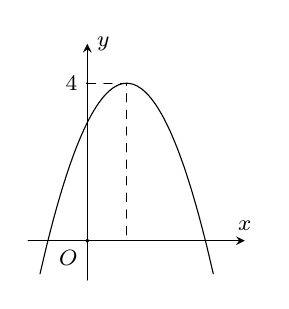
\begin{tikzpicture}[scale=0.5, line join=round, font=\footnotesize, line cap=round,>=stealth]
			\draw[-stealth](-1.5,0)--(4,0) node[above]{$x$}; 
			\draw[-stealth](0,-1.)--(0,5.) node[right]{$y$};		
			\draw[fill=black](0,0)circle (1pt)node[below left]{$O$};
			\draw[dashed](0,4)-|(1,0);
			\foreach \x/\g in {4/180}\fill[black] (0,\x) circle (1pt)+(\g:.4)node{$\x$};		
			\draw[smooth,domain=-1.2:3.2] plot (\x,{-(\x)^2+2*\x+3});
		\end{tikzpicture}
	}
	\loigiai{
		Ta có $\big|f(x)\big|=m-1\Leftrightarrow\heva{&m-1\geq0\\&\hoac{&f(x)=m-1\\&f(x)=-(m-1).}}$\\
		Phương trình có $4$ nghiệm phân biệt khi và chỉ khi
		$$\heva{&m-1>0\\&m-1<4\\&-(m-1)<4}\Leftrightarrow\heva{&m>1\\&m<5} \Leftrightarrow 1<m<5.$$
	}
\end{ex}

\begin{ex}%[0D2G2-3]%[Dự án đề kiểm tra HKII NH22-23- Dương Phước Sang]%[THPT Yên Mô B - Ninh Bình]
	Trong dịp Tết năm nay, một cửa hàng bánh kẹo dự định kinh doanh bánh thương hiệu X với hai loại bánh kí hiệu là loại I (cao cấp), loại II (bình dân). Số vốn để nhập không vượt quá $80$ triệu đồng. Giá nhập vào và dự kiến bán ra như sau:
	\begin{center}
		\begin{tabular}{|l|c|c|}
			\hline \multicolumn{1}{|c|}{ Giá } & Bánh loại I & Bánh loại II \\
			\hline Giá mua vào & $200$ nghìn đồng/hộp & $100$ nghìn đồng/hộp \\
			\hline Giá bán ra & $240$ nghìn đồng/hộp & $125$ nghìn đồng/hộp \\
			\hline
		\end{tabular}
	\end{center}
	Cửa hàng khảo sát được tổng nhu cầu của thị trường sẽ không vượt quá $500$ hộp cả hai loại bánh. Nếu bán hết số hàng sẽ nhập, số tiền lãi lớn nhất mà cửa hàng có thể thu được là
	\choice
	{$16$ triệu đồng}
	{\True $17$ triệu đồng}
	{$18$ triệu đồng}
	{$20$ triệu đồng}
	\loigiai{
		\immini{
			Gọi $x$, $y$ lần lượt là số sản phẩm loại I và loại II nhập vào ($x\geq0$, $y\geq0$).\\
			Ta có hệ bất phương trình\\ $\heva{&200\,000x+100\,000y\leq 80\,000\,000\\&x+y\leq500\\&x\geq0\\&y\geq0}\Leftrightarrow \heva{&2x+y\leq 800&(1)\\&x+y\leq500&(2)\\&x\geq0&(3)\\&y\geq0&(4)}$\\
			Bờ của $(1)$ là $d_1\colon 2x+y=800$, bờ của $(2)$ là $d_2\colon x+y=500$.\\
			Gọi $A=d_1\cap d_2$\\
			$\heva{&2x+y=800\\&x+y=500}\Leftrightarrow\heva{&x=300\\&y=200}\Rightarrow A(300;200)$.\\
			$B=d_1\cap Ox\Rightarrow B(400;0)$; $C=d_2\cap Oy\Rightarrow C(0;500)$.\\
			Lợi nhuận là $F(x;y)=40\,000x+25\,000y$.
		}{
			\begin{tikzpicture}[scale=0.75, line join=round, font=\footnotesize, line cap=round,>=stealth]
				\fill[pattern=north east lines,opacity=0.5](-1,-1)--(0,-1)--(0,9)--(-1,9)--cycle;
				\fill[pattern=north east lines,opacity=0.5](-1,-1)--(7,-1)--(7,0)--(-1,0)--cycle;
				\fill[pattern=north east lines,opacity=0.5](0,8)--(4,0)--(7,0)--(7,3)--(2.2,9)--(0,9)--cycle;
				\fill[pattern=north east lines,opacity=0.5](0,5)--(5,0)--(7,0)--(7,3)--(2.2,9)--(0,9)--cycle;
				\draw[-stealth](-1,0)--(6.1,0) node[above]{$x$ (trăm)}; 
				\draw[-stealth](0,-1)--(0,8.8) node[right]{$y$ (trăm)};		
				\draw[fill=black](0,0)circle (1pt)node[below left]{$O$};
				\draw[dashed](0,2)-|(3,0);
				\foreach \x/\g in {2/180,5/180,8/180}\fill[black] (0,\x) circle (1pt)+(\g:.4)node{$\x$};
				\foreach \x/\g in {3/-90,4/-100,5/-90}\fill[black] (\x,0) circle (1pt)+(\g:.4)node{$\x$};		
				\draw[smooth,domain=-0.5:4.4] plot (\x,{8-2*\x})node[right]{$d_1$};
				\draw[smooth,domain=-0.5:5.5] plot (\x,{5-\x})node[right]{$d_2$};
				\path
				(4,0) coordinate (B)
				(3,2) coordinate (A)
				(0,5) coordinate (C);
				\foreach \x/\g in {A/60,B/70,C/50}\fill[black] (\x) circle (1pt)+(\g:.4)node{$\x$};
				% \draw(0,0)--(3,5) node[right]{$g$};
				% \draw(1,0)--(4,5) node[right]{$d$};
			\end{tikzpicture}
		}
		\noindent Ta thấy $M(100;100)\in (1)$ và  $M(100;100)\in (2)$. Nên miền nghiệm là phần bên trong và các cạnh của tứ giác $OBAC$.\\
		Ta có
		$F(0;0)=40\,000\cdot0+25\,000\cdot0=0$.\\
		$F(400;0)=40\,000\cdot400+25\,000\cdot0=16\,000\,000$.\\
		$F(300;200)=40\,000\cdot300+25\,000\cdot200=17\,000\,000$.\\
		$F(0;500)=40\,000\cdot0+25\,000\cdot500=12\,500\,000$.\\
		Vậy giá lợi nhuận lớn nhất tại điểm $A$. Khi đó lợi nhuận lớn nhất là $17\,000\,000$ đồng.
	}
\end{ex}

\begin{ex}%[0D4K3-4]%[Dự án đề kiểm tra HKII NH22-23- Dương Phước Sang]%[THPT Yên Mô B - Ninh Bình]
	\immini{
		Một kĩ sư thiết kế đường dây điện từ vị trí $A$ đến vị $B$ và từ vị trí $B$ đến vị trí $C$ trên cù lao (như hình bên). Tiền công thiết kế mỗi ki-lô-mét đường dây từ $A$ đến $B$ là $2$ triệu đồng, mỗi ki-lô-mét đường dây từ $B$ đến $C$ là $5$ triệu đồng. Biết $AH=15$ km, $CH=3$ km và tổng tiền công thiết kế là $47$ triệu đồng. Tính tổng số ki-lô-mét đường dây điện đã thiết kế.		
	}{
		\begin{tikzpicture}[scale=0.75, line join=round, font=\footnotesize, line cap=round,>=stealth]
			\path
			(0,0) coordinate (H)
			(2,0) coordinate (B)
			(5,0) coordinate (A)
			(0,3) coordinate (C);
			\foreach \x/\g in {A/0,B/-90,C/90,H/-90}\fill[black] (\x) circle (1pt)+(\g:.4)node{$\x$};
			\draw(A)--(B)--(C);
			\draw[dashed](B)--(H)--(C);
		\end{tikzpicture}
	}
	\choice
	{$15{,}8$ km}
	{\True $16$ km}
	{$17$ km}
	{$18$ km}
	\loigiai{
		Gọi $x$, $y$ lần lượt là độ dài cạnh $AB$ và $BC$ ($0<x<15$, $y>0$, đơn vị: km).\\
		Ta có $2x+5y=47\Leftrightarrow x=\dfrac{47-5y}{2}$.
		Mặt khác 
		\allowdisplaybreaks
		\begin{eqnarray*}
			BC^2=HB^2+HC^2&\Leftrightarrow& y^2=(15-x)^2+3^2\\
			&\Leftrightarrow& y^2=\left(15-\dfrac{47-5y}{2}\right)^2+3^2.\\
			&\Leftrightarrow& y^2=\left(\dfrac{-17+5y}{2}\right)^2+9\\
			&\Leftrightarrow& y^2=\dfrac{289-170y+25y^2}{4}+9\\
			&\Leftrightarrow& 4y^2=289-170y+25y^2+36\\
			&\Leftrightarrow& 21y^2-170y+325=0\\
			&\Leftrightarrow& \hoac{&y=5\Rightarrow x=11\\&y=\dfrac{65}{21}\Rightarrow x=\dfrac{677}{42}>15\text{ (loại)}.}
		\end{eqnarray*}
		Vậy số ki-lô-mét dây điện cần thiết kế là $x+y=11+5=16$ km.
	}
\end{ex}

\begin{ex}%[0H3G2-6]%[Dự án đề kiểm tra HKII NH22-23- Dương Phước Sang]%[THPT Yên Mô B - Ninh Bình]
	Trong mặt phẳng tọa độ $Oxy$, cho hai điểm $A(1;3)$, $B(4;-2)$. Điểm $M$ thay đổi trên trục $Ox$. Véc-tơ $\overrightarrow{u}=2022\overrightarrow{MA}+2023 \overrightarrow{MB}$ có độ dài nhỏ nhất là
	\choice
	{\True $2020$}
	{$2021$}
	{$2022$}
	{$2023$}
	\loigiai{
		Gọi $E(x;y)$ thỏa\\
		\allowdisplaybreaks
		\begin{eqnarray*}
			&&2022\overrightarrow{EA}+2023 \overrightarrow{EB}=\overrightarrow{0}\\
			&\Leftrightarrow&\heva{&2022\left(x_A-x_E\right)+2023\left(x_B-x_E\right)=0\\&2022\left(y_A-y_E\right)+2023\left(y_B-y_E\right)=0}\\
			&\Leftrightarrow&\heva{&x_E=\dfrac{2022x_A+2023x_B}{4045}\\&y_E=\dfrac{2022y_A+2023y_B}{4045}}\\
			&\Leftrightarrow&\heva{&x_E=\dfrac{2022\cdot1+2023\cdot4}{4045}=\dfrac{10114}{4045}\\&y_E=\dfrac{2022\cdot3+2023\cdot(-2)}{4045}=\dfrac{2020}{4045}}
		\end{eqnarray*}
		$\Rightarrow E\left(\dfrac{10114}{4045};\dfrac{2020}{4045}\right)$.
		\begin{eqnarray*}
			\overrightarrow{u}&=&2022\overrightarrow{MA}+2023 \overrightarrow{MB}\\
			&=&2022\left(\overrightarrow{ME}+\overrightarrow{EA}\right)+2023 \left(\overrightarrow{ME}+\overrightarrow{EA}\right)\\
			&=&4045\overrightarrow{ME}+2022\overrightarrow{EA}+2023\overrightarrow{EB}\\
			&=&4045\overrightarrow{ME}
		\end{eqnarray*}
		$\left|\overrightarrow{ME}\right|$ nhỏ nhất khi $M$ là hình chiếu của $E$ lên $Ox\Rightarrow M\left(\dfrac{10114}{4045};0\right)$.\\
		$\overrightarrow{ME}=\left(0;\dfrac{2020}{4045}\right)\Rightarrow\min\left|\overrightarrow{ME}\right|=\dfrac{2020}{4045}$.\\
		$\min\left|\overrightarrow{u}\right|=4045\cdot\dfrac{2020}{4045}=2020$.
	}
\end{ex}

\begin{ex}%[0H3G2-4]%[Dự án đề kiểm tra HKII NH22-23- Dương Phước Sang]%[THPT Yên Mô B - Ninh Bình]
	Trong mặt phẳng tọa độ $Oxy$, cho tam giác $ABC$ biết $A(1;2)$, $B(3;4)$, $C(2;-1)$. Gọi $I(x;y)$ là tâm đường tròn ngoại tiếp của tam giác $ABC$. Giá trị của biểu thức $S=4x+8y$ bằng
	\choice
	{$14$}
	{$22$}
	{\True $35$}
	{$25$}
	\loigiai{
		Gọi $M$ là trung điểm của $AB\Rightarrow M(2;3)$, $N$ là trung điểm của $AC\Rightarrow N\left(\dfrac{3}{2};\dfrac{1}{2}\right)$.\\
		$\overrightarrow{MI}=\left(x-2;y-3\right)$; $\overrightarrow{NI}=\left(x-\dfrac{3}{2};y-\dfrac{1}{2}\right)$; $\overrightarrow{AB}=(2;2)$; $\overrightarrow{AC}=(1;-3)$.\\
		Ta có 
		\begin{eqnarray*}
			&&\heva{&\overrightarrow{AB}\perp\overrightarrow{MI}\\&\overrightarrow{AC}\perp\overrightarrow{NI}}\Leftrightarrow\heva{&\overrightarrow{AB}\cdot\overrightarrow{MI}=0\\&\overrightarrow{AC}\cdot\overrightarrow{NI}=0}
			\Leftrightarrow\heva{&2(x-2)+2(y-3)=0\\&1\left(x-\dfrac{3}{2}\right)-3\left(y-\dfrac{1}{2}\right)=0}\\
			&\Leftrightarrow&\heva{&x+y=5\\&x-3y=0}\Leftrightarrow\heva{&x=\dfrac{5}{4}\\&y=\dfrac{15}{4}.}
		\end{eqnarray*}
		$S=4x+8y=4\cdot\dfrac{5}{4}+8\cdot\dfrac{15}{4}=35$.
	}
\end{ex}

\Closesolutionfile{ans}
%\begin{center}
%	\textbf{ĐÁP ÁN}
%	\inputansbox{10}{ans/ans}	
%\end{center}
\begin{center}
	\textbf{PHẦN 2 - TỰ LUẬN}
\end{center}



\begin{bt}%[0D4Y2-1]%[0D4B3-2]%[Dự án đề kiểm tra HKII NH22-23- Dương Phước Sang]%[THPT Yên Mô B - Ninh Bình]
	Giải bất phương trình và phương trình sau:
	\begin{listEX}[2]
		\item $3x^2-10x+3\leq 0$.
		\item $\sqrt{2x^2-8x+7}=x-2$.
	\end{listEX}
	\loigiai{
		\begin{listEX}
			\item Cho $3x^2-10x+3=0\Leftrightarrow\hoac{&x=\dfrac{1}{3}\\&x=3.}$\\
			Bảng xét dấu
			\begin{center}
				
\begin{tikzpicture}[scale=1]
					\tkzTabInit[nocadre=false,lgt=3,espcl=2.5,deltacl=0.6]{$x$/0.7,$3x^2-10x+3$/0.8}
					{$-\infty$,$\frac{1}{3}$,$3$,$+\infty$}
					\tkzTabLine{,+,0,-,0,+,}
				\end{tikzpicture}	
			\end{center}
			Vậy tập nghiệm của bất phương trình là $S=\left[\dfrac{1}{3};3\right]$.
			\item 
			\begin{eqnarray*}
				&&\sqrt{2x^2-8x+7}=x-2\\
				&\Leftrightarrow&\heva{&x-2\geq 0\\&2x^2-8x+7=(x-2)^2}\\
				&\Leftrightarrow&\heva{&x\geq 2\\&2x^2-8x+7=x^2-4x+4}\\
				&\Leftrightarrow&\heva{&x\geq 2\\&x^2-4x+3=0}\\
				&\Leftrightarrow&\heva{&x\geq 2\\&\hoac{&x=1\text{ (loại)}\\&x=3\text{ (nhận)}.}}\\
			\end{eqnarray*}
			Vậy tập nghiệm của phương trình là $S=\{3\}$.
		\end{listEX}
	}
\end{bt}

\begin{bt}%[0H2B2-3]%[0H3B1-3]%[Dự án đề kiểm tra HKII NH22-23- Dương Phước Sang]%[THPT Yên Mô B - Ninh Bình]
	\indent
	\begin{listEX}
		\item Cho hình bình hành $ABCD$. Chứng minh rằng $\overrightarrow{AC}+\overrightarrow{DB}=2\overrightarrow{AB}$.
		\item Trong mặt phẳng tọa độ $Oxy$, cho tam giác $ABC$ biết $A(1;3)$, $B(2;4)$, $C(5;6)$. Tìm tọa độ điểm $D$ sao cho tứ giác $ABCD$ là hình bình hành.
	\end{listEX}
	\loigiai{
		\begin{listEX}
			\item \immini{Ta có
				\begin{eqnarray*}
					\overrightarrow{AC}+\overrightarrow{DB}&=&\left(\overrightarrow{AB}+\overrightarrow{AD}\right)+\left(\overrightarrow{DA}+\overrightarrow{AB}\right)\\
					&=&\overrightarrow{AB}+\overrightarrow{AD}+\overrightarrow{DA}+\overrightarrow{AB}\\
					&=&\overrightarrow{AB}+\overrightarrow{AB}+\overrightarrow{AD}+\overrightarrow{DA}\\
					&=&2\overrightarrow{AB}.
				\end{eqnarray*}
				
			}{
				\begin{tikzpicture}[scale=1, line join=round, line cap=round,>=stealth]
					\def \r{3}
					\path
					(0,0) coordinate (A)
					(\r,0) coordinate (B)
					(230:0.7*\r) coordinate (D)
					($(B)+(D)$) coordinate (C);
					\draw (A)--(B)--(C)--(D)--(A);
					\foreach \x/\g in {A/150,B/0,C/0,D/180}\fill[black] (\x) circle(1pt)+(\g:0.3)node{$\x$};
				\end{tikzpicture}
			}
			\item Gọi $D(x;y)$ là điểm thỏa $ABCD$ là hình bình hành.\\
			Ta có $\overrightarrow{AD}=\overrightarrow{BC}\Leftrightarrow\heva{&x-1=5-2\\&y-3=6-4}\Leftrightarrow\heva{&x=4\\&y=5.}$\\
			Vậy $D(4;5)$.
		\end{listEX}
		
	}
\end{bt}

\begin{bt}%[0D3Y2-3]%[0D3K2-4]%[Dự án đề kiểm tra HKII NH22-23- Dương Phước Sang]%[THPT Yên Mô B - Ninh Bình]
	Cho hàm số $y=x^2+4x+3$ có đồ thị $(P)$.
	\begin{listEX}
		\item Vẽ đồ thị hàm số trên.
		\item Tìm $m$ để đường thẳng $d\colon y=3x+m$ cắt $(P)$ tại 2 điểm phân biệt $A$, $B$ sao cho $AB=\sqrt{10}$.
	\end{listEX}
	\loigiai{
		\begin{listEX}
			\item Có $a=1>0$ nên hàm số đồng biến trên $\left(-\dfrac{b}{2a};+\infty;\right)=(-2;+\infty;)$,  nghịch biến trên $\left(-\infty;-\dfrac{b}{2a}\right)=(-\infty;-2)$.\\
			Tọa độ đỉnh $\heva{&x=-\dfrac{b}{2a}=-\dfrac{4}{2}=-2\\&y=(-2)^2+4\cdot(-2)+3=-1}\Rightarrow S(-2;-1)$.\\
			Bảng biến thiên
			\begin{center}
				
\begin{tikzpicture}[scale=1]
					\tkzTabInit[nocadre=false,lgt=1.2,espcl=2.5,deltacl=0.6]{$x$/0.7,$y$/2}
					{$-\infty$,$-2$,$+\infty$}
					\tkzTabVar{+/$+\infty$,-/$-1$,+/$+\infty$}
				\end{tikzpicture}	
			\end{center}
			\immini{Bảng giá trị\\ 
				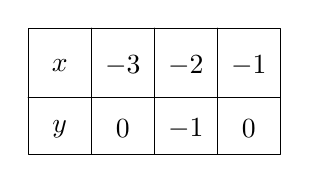
\begin{tikzpicture}[scale=0.8, line join=round, line cap=round,>=stealth]
					\def\a{4} % số nhãn chiều dài
					\def\b{2} % số nhãn chiều cao
					\draw[shift={(-.5,.5)},black] 
					(0,0.1) rectangle +(\a,-\b)
					(0,-1)--+(0:\a) ;
					\foreach \x/ \tren in {0/$x$,1/$-3$,2/$-2$,3/$-1$}
					\draw (\x,0) node{\tren};
					\foreach \y/ \duoi in {0/$y$,1/$0$,2/$-1$,3/$0$}
					\draw (\y,-1) node{\duoi};
					\foreach \z in {.5,1.5,2.5}
					\draw (\z,0.6)--(\z,-1.4) ;
				\end{tikzpicture}
			}{
				\begin{tikzpicture}[scale=0.8, line join=round, font=\footnotesize, line cap=round,>=stealth]
					\draw[->](-4.5,0)--(1.5,0) node[above]{$x$}; 
					\draw[->](0,-1.5)--(0,5) node[right]{$y$} ;		
					\draw[dashed] (-2,0)|-(0,-1);
					\draw[fill=black](0,0)circle (1pt)node[below left]{$O$};
					\foreach \x/\g in {-3/210,-2/110,-1/140}\fill[black] (\x,0) circle (1pt)+(\g:.4)node{$\x$};
					\foreach \x/\g in {-1/0,3/160}\fill[black] (0,\x) circle (1pt)+(\g:.4)node{$\x$};		
					\draw[smooth,domain=-4.3:0.3] plot (\x,{(\x)^2+4*\x+3})node[right]{$(P)$};
				\end{tikzpicture}
			}
			Hàm số đạt giá trị nhỏ nhất $y_{\min}=-1$ khi $x=-2$.
			\item Tìm $m$ để đường thẳng $d\colon y=3x+m$ cắt $(P)$ tại 2 điểm phân biệt $A$, $B$ sao cho $AB=\sqrt{10}$.
			Phương trình hoành độ giao điểm của $(P)$ và $d$
			$$x^2+4x+3=3x+m\Leftrightarrow x^2+x-m=0.\quad(*)$$
			Điều kiện để phương trình $(*)$ có hai nghiệm phân biệt: $\Delta=1+4m>0\Leftrightarrow m>-\dfrac{1}{4}$.\\
			$(P)$ và $d$ cắt nhau tại hai điểm phân biệt $A\left(x_A;y_A\right)$, $B\left(x_B;y_B\right)$ nên $\heva{&y_A=3x_A+m\\&y_B=3x_B+m.}$\\
			Vì $x_A$, $x_B$ là nghiệm của phương trình $(*)$.\\
			Áp dụng định lý Vi-ét: $\heva{&S=x_A+x_B=-1\\&P=x_Ax_B=-m.}$\\
			\begin{eqnarray*}
				AB=\sqrt{10}&\Leftrightarrow&\sqrt{\left(x_B-x_A\right)^2+\left(y_B-y_A\right)^2}=\sqrt{10}\\
				&\Leftrightarrow& \left(x_B-x_A\right)^2+\left(3x_B+m-3x_A-m\right)^2=10\\
				&\Leftrightarrow& 10\left(x_B-x_A\right)^2=10\\
				&\Leftrightarrow& \left(x_B+x_A\right)^2-4x_Bx_A=1\\
				&\Leftrightarrow& (-1)^2-4(-m)=1\\
				&\Leftrightarrow& m=0\text{ (thỏa mãn).}
			\end{eqnarray*}
		\end{listEX}
	}
\end{bt}
